\section{Donut sinh dữ liệu có cấu trúc từ ảnh}
\textcite{kim2022} giới thiệu Donut, một kiến trúc gồm bộ mã hóa ảnh Swin Transformer và bộ giải mã Transformer tự hồi quy. Bộ giải mã nhận một token chỉ định nhiệm vụ và sinh từng token dựa trên biểu diễn ảnh và các token trước đó. Trong bài báo, dữ liệu tổng hợp hỗ trợ tiền huấn luyện khả năng đọc ảnh tài liệu, sau đó mô hình được tinh chỉnh cho các nhiệm vụ như phân tích cấu trúc hóa đơn.

\noindent\begin{minipage}{\textwidth}
\centering
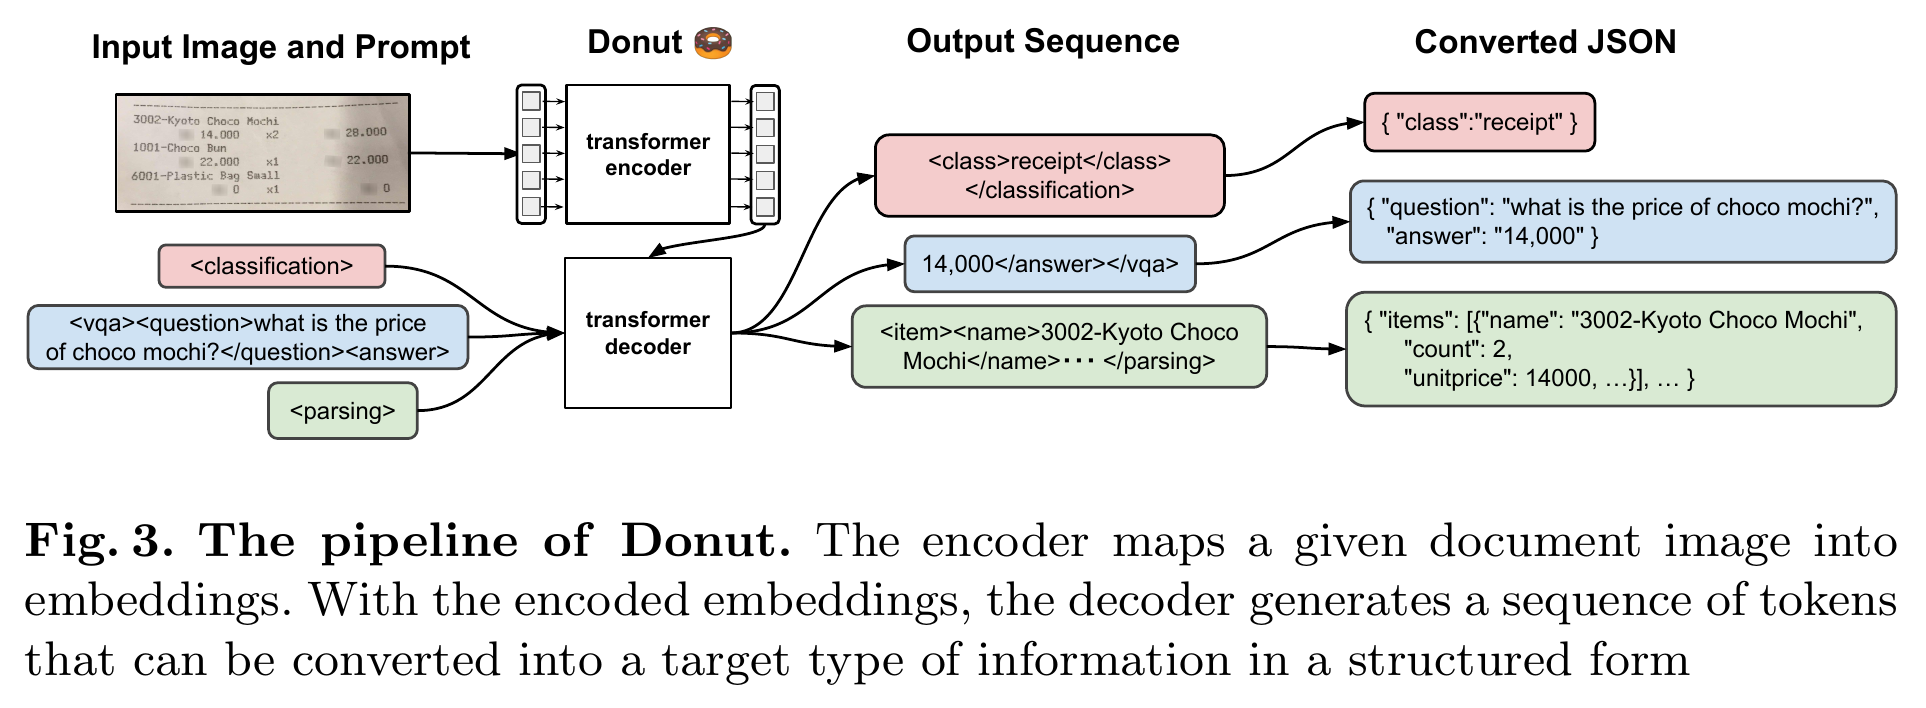
\includegraphics[width=0.94\textwidth,height=7cm,keepaspectratio]{picture/donut-paper-figure-3.png}
\captionof{figure}{Tiền huấn luyện và tinh chỉnh Donut cho các nhiệm vụ tài liệu}
{\small (Nguồn: Hình 3 của \textcite{kim2022})\par}
\end{minipage}

Nhóm sử dụng ảnh hóa đơn và token nhiệm vụ ứng với bộ dữ liệu. Đầu ra huấn luyện của nhóm là chuỗi JSON. Bài báo minh họa cách tuần tự hóa dữ liệu thành chuỗi thẻ và chuyển ngược về dạng cấu trúc.

